\documentclass[]{article}

%opening
\title{Planning and Risks}
\author{Exam Number: B032374}
\date{\today}

\usepackage[parfill]{parskip}
\usepackage{pgfgantt}
\usepackage{multicol}
\usepackage{tikz}
\usepackage{pgfplots}

\usepackage{graphicx}
\graphicspath{ {images/} }

\begin{document}

\maketitle

\section{Introduction}

Investigate the effect of activation function on a multi-layer neural network.

This part of the report investigates how the choice of activation function affectstraining set performance of a small multi-layer model. Three transformation functions withdifferent characteristics were tested and evaluated.
Additionally

How does the number of hidden layer and hidden units affect the training of a deep neural network?



\section{Methodology}

\subsection{The Core Model}

A simple three-layer model with was chosen for this study. The weights for the fully connected layers were initialized by a random distribution, using the tf.truncated\_normal function from TensorFlow. Then the biases are initialized with tf.zeros to ensure they start with all zero values, and their shape is simply the number of units in the layer to which they connect. In addition, L2 Regularisation, with penalty term 0.0001, was used with each affine layer. A simple schematic representation of the model can be seen in Figure \ref{part1-model}.

The model was trained on image classification, using labelled images from the CIFAR-10 data set. To accommodate the CIFAR-10 image size of 32x32, and three color channels, the model's input dimension was 3x1024. Furthermore the model used hidden layers of dimension 200, and a 10 dimensional softmax output layer. A cross entropy error function was used with the model.

\begin{figure}[h]
	\includegraphics[width=\textwidth]{model_1}
	\caption{Showing a visual representation of the model used, from TensorBoard.}
	\label{part1-model}
	\centering
\end{figure}

relu
elu
sigmoid
tanh

\begin{figure}[h]
	\centering
	\begin{tikzpicture}
	\begin{axis}[
	axis lines = left,
	xlabel = $x$,
	ylabel = {$f(x)$},
	xmin=-4, xmax=4,
	ymin=-2, ymax=3,
	]
	\addplot[color=red]{max(0, x)};
	\end{axis}
	\end{tikzpicture}
	\begin{tikzpicture}
	\begin{axis}[
	axis lines = left,
	xlabel = $x$,
	ylabel = {$f(x)$},
	xmin=-4, xmax=4,
	ymin=-2, ymax=3,
	]
	\addplot[color=blue]{tanh(x)};
	\end{axis}
	\end{tikzpicture}
	\begin{tikzpicture}
	\begin{axis}[
	axis lines = left,
	xlabel = $x$,
	ylabel = {$f(x)$},
	xmin=-4, xmax=4,
	ymin=-2, ymax=3,
	]
	\addplot[color=brown]{1/(1+e^(-x))};
	\end{axis}
	\end{tikzpicture}
	\caption{Showing the plots of the transformation functions. Left: Relu. Middle: Tanh. Right: Sigmoid.}
	\label{part1-plots}
\end{figure}


\subsection{The Experiments}


\subsubsection{Activation Functions}

Three non-linear transformation functions were compared. The logistic sigmoid $f(x)=\frac{1}{1+e^{-x}}$, the hyperbolic tangent $f(x)=tanh(x)$ and the rectified linear (ReLu) $f(x)=max(0,x)$.

\begin{figure}[h]
	\centering
	\begin{tikzpicture}
	\begin{axis}[
	axis lines = left,
	xlabel = $x$,
	ylabel = {$f(x)$},
	xmin=-4, xmax=4,
	ymin=-2, ymax=3,
	]
	\addplot[color=red]{max(0, x)};
	\end{axis}
	\end{tikzpicture}
	\begin{tikzpicture}
	\begin{axis}[
	axis lines = left,
	xlabel = $x$,
	ylabel = {$f(x)$},
	xmin=-4, xmax=4,
	ymin=-2, ymax=3,
	]
	\addplot[color=blue]{tanh(x)};
	\end{axis}
	\end{tikzpicture}
	\begin{tikzpicture}
	\begin{axis}[
	axis lines = left,
	xlabel = $x$,
	ylabel = {$f(x)$},
	xmin=-4, xmax=4,
	ymin=-2, ymax=3,
	]
	\addplot[color=brown]{1/(1+e^(-x))};
	\end{axis}
	\end{tikzpicture}
	\caption{Showing the plots of the transformation functions. Left: Relu. Middle: Tanh. Right: Sigmoid.}
	\label{part1-plots}
\end{figure}

Both the hyperbolic tangent and the sigmoid functions compress their input values between (-1, 1) and (0, 1) respectively. A result of such saturation will cause their gradients to approach zero, which means smaller parameter changes and slower training. Two key differences between the two are that the hyperbolic tangent allows for both positive and negative outputs, and that the hyperbolic tangent is centered around zero. The sigmoid transformation function is centered around 0.5, which is not ideal when training models.

The ReLu transformation function looks and behaves quite differently from the two before mentioned alternatives, see Figure \ref{part1-plots}. The ReLu function has a constant gradient of 1 for activations greater than zero, and it will not suffer from diminishing gradients. It can however kill all the units, by responding to everything with 0. Furthermore, as it is unbounded, it will be more sensitive to learning rates than the sigmoid and hyperbolic tangent.

In addition to ReLu, the Exponential Linear Unit (ELU), was also tested \cite{elu}. 

ELU

\subsubsection{Hidden Layers}

depths 1 2 4 5
widths 50 100 200 400


\subsubsection{Learning Rate Schedules}

The third experiment investigates the implementation of a time-dependent learning rate schedule. This report uses an exponential learning rate schedule  
\begin{equation} \label{eq:1}
\eta(t) = \eta_{0} \gamma ^{(t / t_{decay})}
\end{equation}
where \(\eta(t)\) is the learning rate after t steps, \(\eta_{0}\) the initial learning rate and \(\gamma\) is the decay rate. \(t_{decay}\) is the number of steps required for one decay-cycle. The value of \(\gamma\) and \(t_{decay}\) determine the rate of decay of the learning rate. 

The learning schedule was implemented using already built functionality from TensorFlow. The optimiser updates the step, which changes the learning rate, which goes back into the optimiser.  The tf.train.exponential\_decay

\begin{figure}[h]
	\includegraphics[width=\textwidth]{model_2}
	\caption{Showing a visual representation of the learning rate schedule, from TensorBoard.}
	\label{model_2}
	\centering
\end{figure}

The decay rate and the decay steps were only changed during some initial testing, and were set to 0.96 and 10,000 respectively. The initial learning rates used were 0.02, 0.03, 0.05, 0.07 and 0.1. 

\subsection{The Training}

The model was trained for 40 epochs, or 32,000 steps, with batch size of 50, for all four activation functions. The Adam optimiser, with learning rate of 0.01 was used for the training. The Summary Operator from TensorFlow was used to record the data from the experiments. The training data was recorded every step, whereas the validation data was recorded every 100 steps.

\section{Results and Discussion}

\subsubsection{Activation F}

\begin{figure}[h]
	\centering
	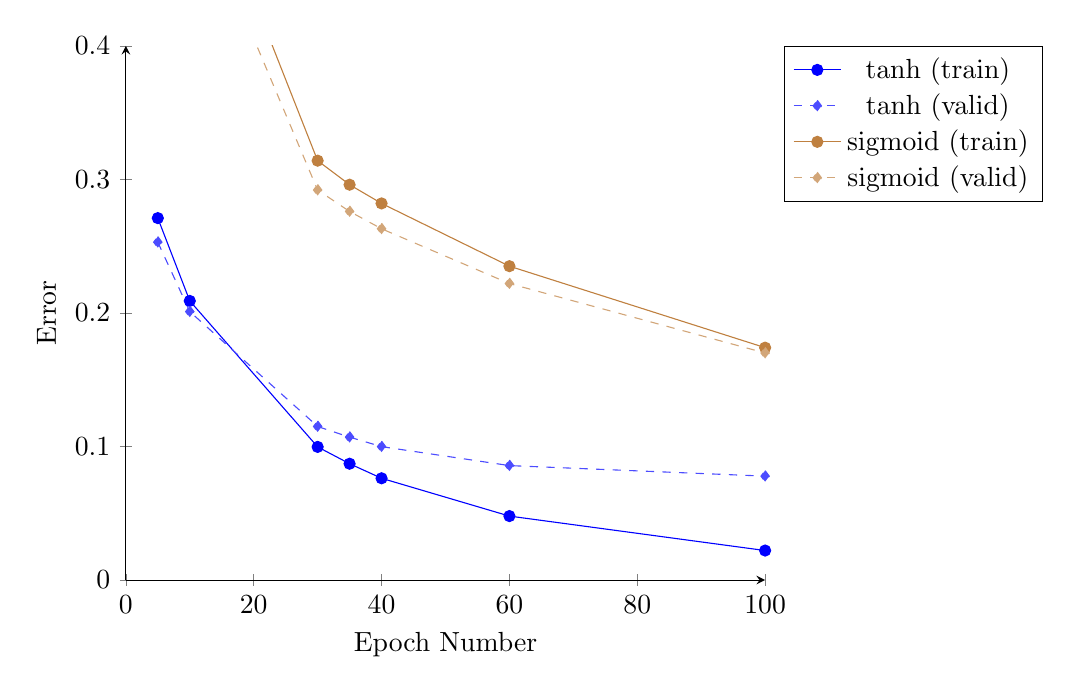
\begin{tikzpicture}
	\begin{axis}[
	width=0.8\textwidth,
	axis lines = left,
	xlabel = {Epoch Number},
	ylabel = {Error},
	xmin=0, xmax=100,
	ymin=0, ymax=0.4,
	legend pos=outer north east
	]
	
	\addplot[color=blue,mark=*]
	coordinates {
		(5, 2.71e-01)(10, 2.09e-01)(30, 9.97e-02)(35, 8.71e-02)(40, 7.62e-02)(60, 4.79e-02)(100, 2.21e-02)
	};
	\addlegendentry{tanh (train)};
	\addplot[dashed, color=blue!70,mark=diamond*]
	coordinates {
		(5, 2.53e-01)(10, 2.01e-01)(30, 1.15e-01)(35, 1.07e-01)(40, 9.99e-02)(60, 8.57e-02)(100, 7.78e-02)
	};
	\addlegendentry{tanh (valid)};
	
	\addplot[color=brown,mark=*]
	coordinates {
		(5, 1.03e+00)(10, 5.57e-01)(30, 3.14e-01)(35, 2.96e-01)(40, 2.82e-01)(60, 2.35e-01)(100, 1.74e-01)
	};
	\addlegendentry{sigmoid (train)};
	\addplot[dashed, color=brown!70,mark=diamond*]
	coordinates {
		(5, 9.97e-01)(10, 5.19e-01)(30, 2.92e-01)(35, 2.76e-01)(40, 2.63e-01)(60, 2.22e-01)(100, 1.70e-01)
	};
	\addlegendentry{sigmoid (valid)};
	
	\end{axis}
	\end{tikzpicture}
	
	\caption{Showing the evolution of the error function values across the training epochs, for the momentum learning rule.}
	\label{part1-error}
\end{figure}


\begin{figure}[h]
	
	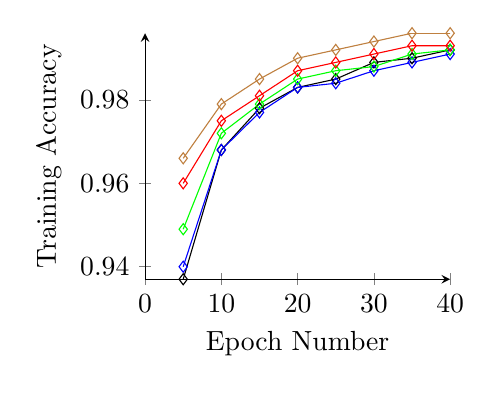
\begin{tikzpicture}
	\begin{axis}[
	width=0.45\textwidth,
	axis lines = left,
	xlabel = {Epoch Number},
	ylabel = {Training Accuracy},
	xmin=0, xmax=40
	]
	\addplot[color=black,mark=diamond]
	coordinates {
		(5, 0.937)(10, 0.968)(15, 0.978)(20, 0.983)(25, 0.985)(30, 0.989)(35, 0.99)(40, 0.992)
	};
	\addplot[color=blue,mark=diamond]
	coordinates {
		(5, 0.94)(10, 0.968)(15, 0.977)(20, 0.983)(25, 0.984)(30, 0.987)(35, 0.989)(40, 0.991)
	};
	\addplot[color=green,mark=diamond]
	coordinates {
		(5, 0.949)(10, 0.972)(15, 0.979)(20, 0.985)(25, 0.987)(30, 0.988)(35, 0.991)(40, 0.992)
	};
	\addplot[color=red,mark=diamond]
	coordinates {
		(5, 0.96)(10, 0.975)(15, 0.981)(20, 0.987)(25, 0.989)(30, 0.991)(35, 0.993)(40, 0.993)
	};
	\addplot[color=brown,mark=diamond]
	coordinates {
		(5, 0.966)(10, 0.979)(15, 0.985)(20, 0.99)(25, 0.992)(30, 0.994)(35, 0.996)(40, 0.996)
	};
	\end{axis}
	\end{tikzpicture}
	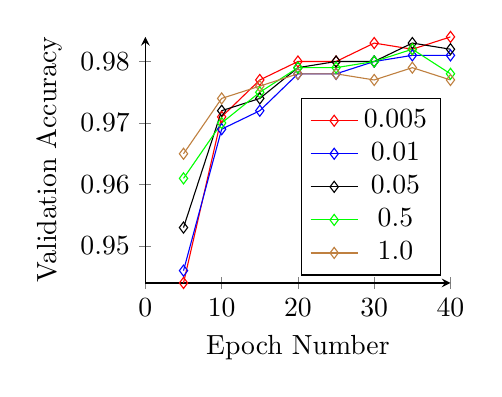
\begin{tikzpicture}
	\begin{axis}[
	width=0.45\textwidth,
	axis lines = left,
	xlabel = {Epoch Number},
	ylabel = {Validation Accuracy},
	xmin=0, xmax=40,
	legend pos=south east,
	]
	\addplot[color=red,mark=diamond]
	coordinates {
		(5, 0.944)(10, 0.971)(15, 0.977)(20, 0.980)(25, 0.980)(30, 0.983)(35, 0.982)(40, 0.984)
	};
	\addlegendentry{0.005};
	\addplot[color=blue,mark=diamond]
	coordinates {
		(5, 0.946)(10, 0.969)(15, 0.972)(20, 0.978)(25, 0.978)(30, 0.98)(35, 0.981)(40, 0.981)
	};
	\addlegendentry{0.01};
	\addplot[color=black,mark=diamond]
	coordinates {
		(5, 0.953)(10, 0.972)(15, 0.974)(20, 0.979)(25, 0.98)(30, 0.98)(35, 0.983)(40, 0.982)
	};
	\addlegendentry{0.05};
	\addplot[color=green,mark=diamond]
	coordinates {
		(5, 0.961)(10, 0.97)(15, 0.975)(20, 0.979)(25, 0.979)(30, 0.98)(35, 0.982)(40, 0.978)
	};
	\addlegendentry{0.5};
	\addplot[color=brown,mark=diamond]
	coordinates {
		(5, 0.965)(10, 0.974)(15, 0.976)(20, 0.978)(25, 0.978)(30, 0.977)(35, 0.979)(40, 0.977)
	};
	\addlegendentry{1.0};
	\end{axis}
	\end{tikzpicture}
	
	\caption{Showing the evolution of the classification accuracy across the training epochs, for the different scaling values of the kernel.}
	\label{part3-acc}
	\centering
\end{figure}

\section{Conclusion}

\section{Future Work}

\clearpage
\medskip
\bibliographystyle{IEEEtran}
\bibliography{ref.bib}

\end{document}
